\documentclass[conference]{IEEEtran}
\IEEEoverridecommandlockouts

\usepackage{cite}
\usepackage{amsmath,amssymb,amsfonts,amsthm}
\usepackage{graphicx}
\usepackage{booktabs}
\usepackage{xcolor}
\usepackage{url}
\usepackage[hidelinks]{hyperref}
\usepackage{orcidlink}

\newtheorem{theorem}{Theorem}
\newtheorem{proposition}{Proposition}
\newtheorem{lemma}{Lemma}
\newtheorem{corollary}{Corollary}
\theoremstyle{definition}
\newtheorem{assumption}{Assumption}
\newcommand{\ket}[1]{\left|#1\right\rangle}
\newcommand{\cpla}{CPLA}

\begin{document}

\title{Quantum Attention Is a Kernel, Not (Yet) a Speedup:\\Training-Cost Bounds and Linear-Time Recall\\for Transformers}

\author{\IEEEauthorblockN{Chandra Sekhar Singuru\,\orcidlink{0009-0004-0219-1960}}
\IEEEauthorblockA{\textit{Independent Researcher}\\
Long Beach, CA, USA\\
sekharc669@gmail.com\\
ORCID: 0009-0004-0219-1960}
}

\maketitle

\begin{abstract}
Quantum self-attention computes Transformer attention scores as overlaps of quantum states. We ask whether this is worth doing on quantum hardware, and what classical Transformers should borrow from it. We measure two scaling laws of the fidelity attention score: its mean decays as $2^{-n}$ and its gradient variance as approximately $4^{-n}$ in the number of qubits $n$ (fitted rate $3.97$, 95\% interval $3.85$--$4.06$). Combining them with Bernoulli shot noise and parameter-shift gradients, we prove a lower bound on the shots per training step and a closed-form condition for any quantum advantage over exact classical simulation. The minimum training time inside any advantage regime scales as $\kappa^2/R_s^2$, where $\kappa$ is the number of circuits per token pair and $R_s$ the shot rate. With parameter-shift gradients this is at least 64 years per step on one sequence at $10^4$ shots/s and 1.5 days at $10^6$. A sweep over 144 hardware scenarios shows that training becomes practical only if three conditions hold together: a backpropagation-like gradient estimator, which no known construction provides for this circuit; coherent aggregation of gradients across token pairs; and at least $10^5$ shots/s. On the classical side, we give an exact $3^n$-dimensional feature map for the cosine-product kernel that underlies fidelity attention and evaluate the resulting linear-time layer, CPLA, on multi-query associative recall in two-layer Transformers. At an identical 81-dimensional state, CPLA retains 86\% recall at 16 key-value pairs where standard linear attention falls to 12.5\%, and it far exceeds Performer; it trails the second-order Taylor kernel of Based by 4--13 points at moderate load, and no fixed-state method survives 32 pairs. Quantum attention thus contributes a useful multiplicative kernel; a speedup would require gradient estimators and shot rates beyond those available today.
\end{abstract}

\begin{IEEEkeywords}
Transformers, attention mechanism, linear attention, associative recall, quantum machine learning, quantum kernels, barren plateaus, computational cost
\end{IEEEkeywords}

% ===========================================================================
\section{Introduction}
% ===========================================================================

Attention is the most expensive part of a Transformer~\cite{vaswani2017attention}. Its pairwise scores cost time quadratic in the sequence length $N$, which has motivated a large body of work on efficient attention: kernel views of attention~\cite{tsai2019dissection}, linear attention~\cite{katharopoulos2020linear}, random-feature approximations~\cite{choromanski2021performer} and re-weighted linear kernels~\cite{qin2022cosformer}. A recurring finding is that efficient models struggle with \emph{associative recall}, retrieving a value seen earlier in the context given its key~\cite{arora2024zoology,arora2024based}.

Quantum self-attention has been proposed as another route~\cite{li2024qsann,zhao2024qksan,chen2024qmsan,pecilli2026overlap,xu2026higher,zhang2025survey}. Tokens are encoded as quantum states, and attention scores are computed from state overlaps on a quantum processor. Our earlier work~\cite{singuru2026fidelity} showed that, for angle-encoded states, the fidelity score equals a classical cosine-product (CP) kernel, and that any fidelity attention admits an exact linear-time classical evaluation. That result leaves two questions that matter to practitioners building Transformers.

\begin{enumerate}
  \item \textbf{Is training quantum attention on hardware ever worth its cost?} Existing analyses estimate shot counts for evaluating quantum kernels~\cite{miroszewski2024shots,thanasilp2024concentration}, but not the cost of \emph{training} an attention layer, where every token pair needs gradient estimates.
  \item \textbf{What, if anything, should classical Transformers borrow?} If the useful part of quantum attention is a classical kernel, does that kernel help on the recall tasks where efficient attention is known to fail?
\end{enumerate}

\noindent Our contributions are:
\begin{itemize}
  \item \textbf{Two measured scaling laws} for the quantum fidelity score: its mean decays as $2^{-n}$ and its gradient variance as $\approx 4^{-n}$ in the number of qubits $n$ (Section~\ref{sec:scaling}).
  \item \textbf{A training-cost theorem.} Accounting for Bernoulli shot noise, the number of circuits per gradient and the most quantum-favourable aggregation of gradients, we derive a lower bound on the shots per training step and a closed-form condition for any quantum advantage over exact classical simulation (Section~\ref{sec:cost}).
  \item \textbf{A quantitative verdict.} With parameter-shift gradients, any regime in which quantum hardware is cheaper than exact classical simulation needs at least 1.5 days per training step on a single sequence at $10^6$ shots/s and 64 years at $10^4$; an idealized gradient estimator would shorten this to seconds at $10^6$ shots/s, and we quantify both cases over 144 hardware scenarios.
  \item \textbf{An exact $3^n$-dimensional feature map} for the CP kernel, smaller than the $4^n$ of~\cite{singuru2026fidelity}, and an evaluation of the resulting linear-time layer (\cpla) on multi-query associative recall against Based~\cite{arora2024based}, linear attention and Performer (Section~\ref{sec:recall}).
\end{itemize}

% ===========================================================================
\section{Related Work}
% ===========================================================================

\subsection{Efficient Attention and Recall}
Tsai \emph{et al.}~\cite{tsai2019dissection} interpret attention as kernel smoothing, which lets the similarity function be studied apart from the projections around it. Linear attention~\cite{katharopoulos2020linear} uses a positive feature map so that the sum over keys can be reassociated, giving cost linear in $N$; Performer~\cite{choromanski2021performer} estimates softmax attention through positive random projections, and cosFormer~\cite{qin2022cosformer} modulates scores with a cosine of token distance. Zoology~\cite{arora2024zoology} introduced multi-query associative recall (MQAR) and showed that efficient architectures lag attention on it. Based~\cite{arora2024based} pairs a small sliding window with linear attention whose features expand $\exp(q\cdot k)$ to second order, trading recurrent-state size for recall.

\subsection{Quantum Self-Attention}
QSANN~\cite{li2024qsann} scores queries and keys from single Pauli-$Z$ measurements; QKSAN~\cite{zhao2024qksan} uses quantum kernel overlaps; QMSAN~\cite{chen2024qmsan} uses swap tests between mixed states; Pecilli and Rosati~\cite{pecilli2026overlap} drop the softmax to obtain gate complexity linear in sequence length; and Xu \emph{et al.}~\cite{xu2026higher} build higher-order interactions from expectation read-outs. A recent survey~\cite{zhang2025survey} observes that scoring token pairs one at a time on a quantum device does not escape the $N^2$ cost of classical attention. Our prior work~\cite{singuru2026fidelity} reduced fidelity attention exactly to classical computation. None of these works analyses the end-to-end cost of training.

\subsection{Cost and Trainability of Quantum Kernels}
Fidelity kernels~\cite{havlicek2019supervised} can concentrate exponentially, so that distinguishing inputs needs exponentially many shots~\cite{thanasilp2024concentration}. Slattery \emph{et al.}~\cite{slattery2023evidence} found that well-tuned fidelity kernels are approximated by classical kernels, and Bowles \emph{et al.}~\cite{bowles2024benchmarking} found no systematic advantage of quantum models in benchmarks. Miroszewski \emph{et al.}~\cite{miroszewski2024shots} estimated the shots needed to \emph{evaluate} quantum kernel matrices and compared them with classical simulation, concluding that quantum utility may appear above about 40 qubits. Bowles \emph{et al.}~\cite{bowles2025backprop} showed that circuits with commuting generators admit gradient estimation with far fewer circuits than the parameter-shift rule. Barren plateaus~\cite{mcclean2018barren}, particularly for global observables~\cite{cerezo2021cost}, make gradients vanish exponentially, and their provable absence often coincides with classical simulability~\cite{cerezo2025simulability}. We add the attention-specific, training-time analysis: quadratic pairs, gradient estimation, and comparison against the linear-time classical reduction.

% ===========================================================================
\section{Background: Quantum Fidelity Attention}
\label{sec:prelim}
% ===========================================================================

Each token embedding $x$ is mapped to $n$ angles $\phi(x)=\pi\tanh(Ax)$ and encoded as $S(\phi)\ket{0}^{\otimes n}=\bigotimes_k(\cos\frac{\phi_k}{2}\ket{0}+\sin\frac{\phi_k}{2}\ket{1})$. Separate hardware-efficient ansatzes $W_Q$, $W_K$ with $L$ layers of $R_Y$ rotations and CNOT rings give query and key states, and the score is the fidelity
\begin{equation}
s_{ij}=\left|\langle\psi_K(x_j)|\psi_Q(x_i)\rangle\right|^2,
\end{equation}
estimated on hardware with a compute--uncompute circuit whose all-zeros outcome probability equals $s_{ij}$~\cite{singuru2026fidelity}. Each score circuit has $P=2n+2nL=2n(L+1)$ rotation angles, and gradients follow the parameter-shift rule $\partial s/\partial a=\frac12[s(a+\frac{\pi}{2})-s(a-\frac{\pi}{2})]$~\cite{schuld2019gradients}, so a training step evaluates $\kappa=1+2P$ circuits per token pair. We keep $\kappa$ general below, since better gradient estimators can lower it~\cite{bowles2025backprop}.

Without an ansatz the score is the CP kernel $s_{ij}=\prod_k\cos^2\!\big((\phi_{ik}-\phi_{jk})/2\big)$, and with any ansatz $s_{ij}$ can still be written as a dot product of $4^n$-dimensional feature vectors~\cite{singuru2026fidelity}. We sharpen the feature dimension for the CP kernel.

\begin{proposition}[Exact $3^n$ feature map]\label{prop:three}
Let $f(\phi)=\bigotimes_{k=1}^{n}\frac{1}{\sqrt2}\,[1,\cos\phi_k,\sin\phi_k]\in\mathbb{R}^{3^n}$. Then $\prod_k\cos^2\!\big((a_k-b_k)/2\big)=\langle f(a),f(b)\rangle$.
\end{proposition}
\begin{proof}
For one feature, $\cos^2\frac{a-b}{2}=\frac12\big(1+\cos(a-b)\big)=\frac12\big(1+\cos a\cos b+\sin a\sin b\big)$, the inner product of $\frac{1}{\sqrt2}[1,\cos a,\sin a]$ and $\frac{1}{\sqrt2}[1,\cos b,\sin b]$. Inner products of tensor products factorize.
\end{proof}

\noindent The map reduces the linear-time state from $4^n$ to $3^n$ per head (81 instead of 256 for $n=4$), and allows separate query and key angle projections while preserving exact linear-time evaluation. We call the resulting layer cosine-product linear attention (\cpla).

% ===========================================================================
\section{Two Scaling Laws of the Fidelity Score}
\label{sec:scaling}
% ===========================================================================

\begin{figure}[t]
\centering
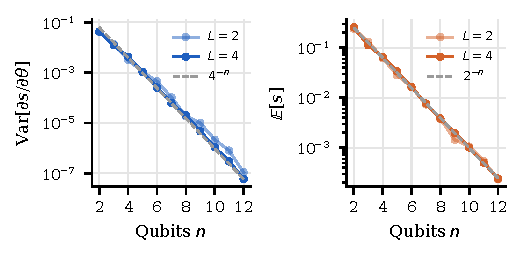
\includegraphics[width=\columnwidth]{figures/scaling.pdf}
\caption{Gradient variance (left) and mean score (right) of the fidelity attention score at uniformly random parameters, 400 samples per point, for $L=2$ and $L=4$ ansatz layers. Dashed lines show $4^{-n}$ and $2^{-n}$.}
\label{fig:scaling}
\end{figure}

We measured, for $n=2$ to $12$ and $L\in\{2,4\}$, the mean score $p(n)=\mathbb{E}[s]$ and the gradient variance $V(n)=\operatorname{Var}[\partial s/\partial\theta_{Q,1}]$ over uniformly random inputs and parameters, using an exact statevector simulator validated against the Qiskit Estimator~\cite{qiskit2024} to within $10^{-15}$. Fitting $\log$-linear models for $n\ge4$ gives (95\% bootstrap intervals in parentheses):
\begin{itemize}
  \item $p(n)\propto 1.99^{-n}$ ($L=2$) and $2.01^{-n}$ ($L=4$), matching the Haar value $\mathbb{E}|\langle\psi|\varphi\rangle|^2=2^{-n}$;
  \item $V(n)\propto 3.53^{-n}$ ($3.27$--$3.83$) for $L=2$ and $3.97^{-n}$ ($3.85$--$4.06$) for $L=4$.
\end{itemize}
The deeper circuit reaches the $4^{-n}$ rate expected of a global observable on an approximate 2-design~\cite{mcclean2018barren,cerezo2021cost}. Fig.~\ref{fig:scaling} shows both laws. They are the inputs to the cost analysis, and we state their extrapolation beyond 12 qubits as an explicit assumption.

\begin{assumption}\label{ass:scaling}
For the register sizes considered, $p(n)=c_p\,r_p^{\,n}$ and $V(n)=a\,r_V^{\,n}$ with the fitted constants, and a typical per-pair gradient has magnitude $\sqrt{V(n)}$.
\end{assumption}

% ===========================================================================
\section{The Cost of Training Fidelity Attention}
\label{sec:cost}
% ===========================================================================

We compare one training step (forward and backward) on one sequence of $N$ tokens. Let $R_s$ be the hardware shot rate, $F$ the classical floating-point rate, $d$ the value width and $g=n(L+1)$ the gates per state.

\begin{lemma}[Shot noise]\label{lem:noise}
A score estimated from $S$ shots has variance $p(1-p)/S$, and the parameter-shift estimate $\hat g=\frac12(\hat s_+-\hat s_-)$ has variance $p(1-p)/(2S)$.
\end{lemma}
\begin{proof}
Each shot is a Bernoulli trial with success probability $s\approx p$. The two shifted estimates are independent, so $\operatorname{Var}\hat g=\frac14\cdot 2\,p(1-p)/S$.
\end{proof}

\begin{theorem}[Quantum shots per step]\label{thm:quantum}
Under Assumption~\ref{ass:scaling}, resolving the gradient of a shared parameter at signal-to-noise ratio at least one requires, per training step,
\begin{equation}
Q\;\ge\;\kappa\,\max\!\Big(N^2,\;\frac{p(1-p)}{2V}\Big)
\label{eq:Q}
\end{equation}
shots, even if per-pair gradients add perfectly coherently.
\end{theorem}
\begin{proof}
Each of the $N^2$ pairs needs at least one shot on each of its $\kappa$ circuits, giving the first term. The aggregated gradient is $G=\sum_{ij}w_{ij}\hat g_{ij}$, with noise variance $\sum w_{ij}^2\,p(1-p)/(2S)$ by Lemma~\ref{lem:noise}. Its signal satisfies $|\mathbb{E}G|^2\le(\sum|w_{ij}|)^2V\le N^2\sum w_{ij}^2V$ by Cauchy--Schwarz, with equality for perfectly coherent pairs. Signal-to-noise at least one therefore needs $S\ge p(1-p)/(2N^2V)$ shots per circuit, and the total is $N^2\kappa S$.
\end{proof}
\noindent If per-pair gradients are incoherent, the signal grows only as $N$ and the second term in \eqref{eq:Q} is multiplied by $N^2$.

\begin{theorem}[Exact classical cost]\label{thm:classical}
Exact forward and backward evaluation of fidelity attention takes at most
\begin{equation}
T_c=\frac{6}{F}\min\!\big(2Ng2^n+2N^2 2^n,\;2Ng2^n+4N\,4^n d\big)
\label{eq:Tc}
\end{equation}
seconds, with memory $2^{n+5}$ bytes for the first (pairwise) algorithm and $8\cdot4^n d$ bytes for the second (linear-time) algorithm.
\end{theorem}
\begin{proof}
Preparing a state costs $g$ gate applications on $2^n$ amplitudes. The pairwise algorithm computes $N^2$ overlaps of length $2^n$, streaming states so that two are held at once. The linear-time algorithm uses the explicit $4^n$ features of~\cite{singuru2026fidelity} with prefix sums. Reverse-mode differentiation costs at most twice the forward pass, giving the factor $6=2\times3$ for multiply-adds over forward and backward.
\end{proof}

\begin{corollary}[Necessary condition for advantage]\label{cor:cond}
If quantum hardware is faster than the pairwise classical algorithm, then $2^n(1+g/N)>\kappa F/(12R_s)$.
\end{corollary}
\begin{proof}
By Theorem~\ref{thm:quantum}, $T_q\ge\kappa N^2/R_s$; by Theorem~\ref{thm:classical}, $T_c\le12(N^2+Ng)2^n/F$. Require $T_q<T_c$.
\end{proof}

\begin{corollary}[Minimum time per step]\label{cor:time}
If $p=2^{-n}$ and $V=a\,4^{-n}$, then whenever quantum hardware beats exact classical simulation with sufficient classical memory,
\begin{equation}
T_q\;\ge\;\frac{\kappa^2\,F}{24\,a\,R_s^{2}}\cdot\frac{N}{N+g}.
\label{eq:Tmin}
\end{equation}
\end{corollary}
\begin{proof}
By Theorem~\ref{thm:quantum}, $T_q\ge\kappa\,p(1-p)/(2VR_s)\approx\kappa\,2^n/(2aR_s)$. Substituting the lower bound on $2^n$ from Corollary~\ref{cor:cond} gives \eqref{eq:Tmin}.
\end{proof}

\noindent The bound grows as $\kappa^2/R_s^2$: both the circuit count and the shot rate enter quadratically, once through the per-pair floor and once through the gradient-shot requirement. With the measured constants for $L=4$ ($a=1.07$), $F=10^{13}$ (one workstation) and parameter-shift gradients ($\kappa=1+2P$), the smallest qualifying register and the resulting bound are $n=36$ and $T_q\ge 64$ years per step at $R_s=10^4$ shots/s; $n=33$ and $198$ days at $10^5$; and $n=29$ and $1.5$ days at $10^6$. A hypothetical estimator returning all gradients from two extra circuits ($\kappa=3$) would lower the bound to $9.8$ hours, $6$ minutes and $3.5$ seconds, at $n=28$, $25$ and $22$. Known constructions of such estimators require commuting generators~\cite{bowles2025backprop}, which the hardware-efficient ansatz used here does not have.

\begin{figure}[t]
\centering
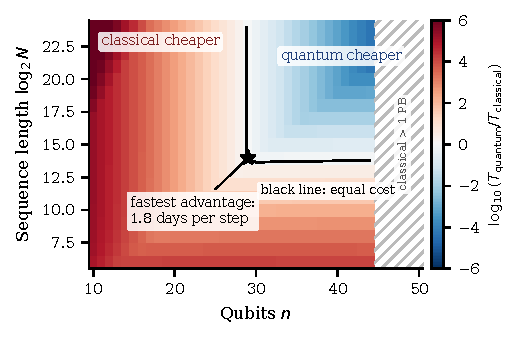
\includegraphics[width=\columnwidth]{figures/feasibility.pdf}
\caption{Ratio of quantum to exact classical training time per step for $L=4$, $R_s=10^6$ shots/s, $F=10^{13}$ flop/s and 1~PB classical memory. Quantum is cheaper only in the upper right, and the fastest such configuration (star) still needs 1.8 days per step on one sequence.}
\label{fig:feasibility}
\end{figure}

\begin{figure}[t]
\centering
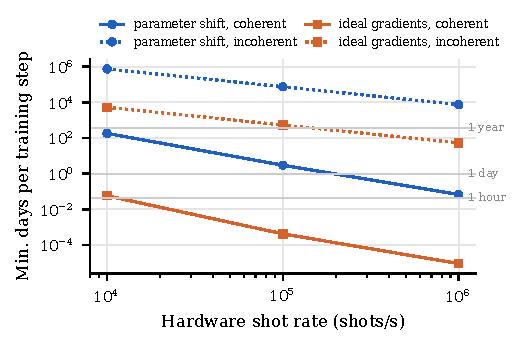
\includegraphics[width=\columnwidth]{figures/shotrate.pdf}
\caption{Minimum time per training step over all configurations where quantum hardware beats exact classical simulation, versus hardware shot rate, for parameter-shift ($\kappa=1+2P$) and idealized ($\kappa=3$) gradient estimators with coherent or incoherent aggregation (sweep over $L$, classical flop rate $10^{13}$--$10^{17}$ and memory $10^{12}$--$10^{15}$ bytes).}
\label{fig:shotrate}
\end{figure}

\textit{Numerical sweep.} To avoid relying on the idealized rates, we evaluated \eqref{eq:Q} and \eqref{eq:Tc} with the fitted constants for every $n\le60$ and $N=2^6$ to $2^{24}$, across 144 scenarios: $L\in\{2,4\}$, $R_s\in\{10^4,10^5,10^6\}$, $F\in\{10^{13},10^{15},10^{17}\}$, memory $\in\{1\,\text{TB},1\,\text{PB}\}$, coherent or incoherent gradients, and $\kappa\in\{1+2P,\,3\}$. Fig.~\ref{fig:feasibility} maps the ratio for one scenario and Fig.~\ref{fig:shotrate} summarizes all of them. A quantum advantage region always exists at large $n$ and $N$. With parameter-shift gradients, the fastest training step inside it takes at least 0.5 years at $10^4$ shots/s, 3.0 days at $10^5$ and 1.6 hours at $10^6$ when gradients aggregate coherently, and 2{,}060, 206 and 20.6 years when they do not; a modest run of $10^4$ steps is out of reach in every such scenario. With the idealized estimator and coherent gradients, the minima fall to 1.4 hours, 37 seconds and 0.8 seconds, so a $10^4$-step run would take 1.6 years, 4.2 days or 2.2 hours; with incoherent gradients they remain 14.7 years, 1.5 years and 54 days per step. Practical training therefore needs a better gradient estimator, coherent gradients and at least $10^5$ shots/s at the same time.

% ===========================================================================
\section{What Transformers Can Borrow: Associative Recall}
\label{sec:recall}
% ===========================================================================

The cost analysis implies that the value of quantum attention, if any, lies in its kernel. We therefore test the classical CP kernel where efficient attention is known to be weak: multi-query associative recall (MQAR)~\cite{arora2024zoology}.

\subsection{Setup}
Each sequence lists $K$ key--value pairs followed by $\min(K,16)$ queries, each a previously seen key; the model must output the paired value. Keys and values come from disjoint vocabularies of 64 tokens each, so chance accuracy is $1/64$. Following Based~\cite{arora2024based}, every model is a two-layer, four-head, pre-norm causal Transformer ($d=64$) whose first layer is sliding-window softmax attention over the last 4 tokens and whose second layer is the attention variant under test. A control with sliding windows in both layers measures how much recall the global layer provides. The second layer is one of:
\begin{itemize}
  \item \textbf{softmax}: full quadratic attention, the reference;
  \item \textbf{\cpla}: linear-time CP kernel with separate 4-angle query and key projections per head, state $3^4=81$ (Proposition~\ref{prop:three});
  \item \textbf{CP softmax}: the same kernel inside a softmax, quadratic;
  \item \textbf{Based}~\cite{arora2024based}: second-order Taylor features of $\exp(q\cdot k/\sqrt{d'})$, state $1+d'+d'^2$ = 73 ($d'=8$) or 273 ($d'=16$);
  \item \textbf{linear elu+1}~\cite{katharopoulos2020linear} with state 81, matched to \cpla;
  \item \textbf{Performer}~\cite{choromanski2021performer} with 64 positive random features.
\end{itemize}
All models train for 2{,}000 steps of AdamW (batch 64, learning rate $10^{-3}$ with one-cycle schedule) on freshly sampled sequences and are evaluated on 2{,}048 held-out sequences, over three seeds for $K\in\{8,16,32\}$. Causality of every variant and exactness of the linear-time forms against their pairwise counterparts were verified numerically.

\begin{figure}[t]
\centering
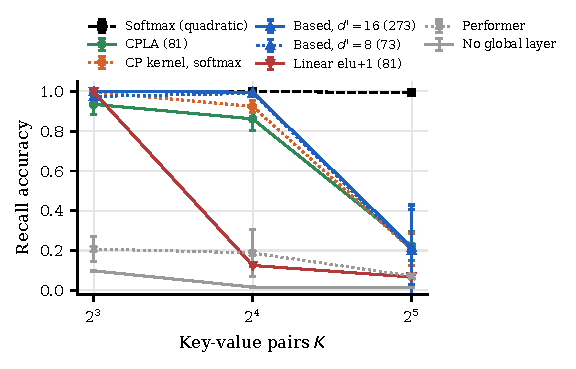
\includegraphics[width=\columnwidth]{figures/recall.pdf}
\caption{Associative recall accuracy versus number of key--value pairs (mean $\pm$ std., 3 seeds). Numbers in parentheses are recurrent-state dimensions per head. At the same state size, \cpla{} (green) retains recall at $K=16$ where linear elu+1 attention (red) collapses.}
\label{fig:recall}
\end{figure}

\begin{table}[t]
\caption{Multi-Query Associative Recall Accuracy (Mean $\pm$ Std., 3 Seeds)}
\label{tab:recall}
\centering
\setlength{\tabcolsep}{3pt}
\begin{tabular}{@{}lcccc@{}}
\toprule
Second layer & State & $K=8$ & $K=16$ & $K=32$ \\
\midrule
Softmax (quadratic)        & $O(N)$ & 1.000$\pm$.000 & 1.000$\pm$.000 & .994$\pm$.002 \\
CP softmax (quadratic)     & $O(N)$ & .997$\pm$.001 & .924$\pm$.029 & .204$\pm$.079 \\
Based, $d'{=}16$           & 273 & .999$\pm$.001 & .997$\pm$.002 & .216$\pm$.189 \\
Based, $d'{=}8$            & 73  & .975$\pm$.032 & .991$\pm$.004 & .203$\pm$.226 \\
\cpla{} (ours)             & 81  & .936$\pm$.054 & .862$\pm$.057 & .222$\pm$.072 \\
Linear elu$+1$             & 81  & .998$\pm$.001 & .125$\pm$.004 & .067$\pm$.002 \\
Performer                  & 64  & .208$\pm$.062 & .187$\pm$.119 & .071$\pm$.002 \\
No global layer            & --  & .098$\pm$.002 & .016$\pm$.001 & .016$\pm$.000 \\
\bottomrule
\end{tabular}
\end{table}

\subsection{Results}
Table~\ref{tab:recall} and Fig.~\ref{fig:recall} give the results. The control without a global layer stays near chance, so recall is performed by the second layer.

\textit{Kernel shape matters at fixed state size.} \cpla{} and linear elu+1 attention carry the same 81-dimensional state per head, yet at $K=16$ \cpla{} recalls 86.2\% of values and elu+1 only 12.5\%, a paired difference of $0.74\pm0.06$ over seeds. \cpla{} also exceeds Performer by 0.68 at $K=16$. The CP kernel multiplies agreement across angle features, so a query matches a key only if all features align, whereas elu+1 features combine additively. Based's second-order Taylor kernel shares this multiplicative character, and both retain recall where additive features fail.

\textit{Based remains stronger.} At moderate load Based outperforms \cpla{} by 4.0 points at $K=8$ and 12.9 at $K=16$ with a smaller 73-dimensional state; at $K=32$ the two are indistinguishable. \cpla{} is also within 6.2 points of its own softmax version, so the linear-time form costs little relative to the kernel itself.

\textit{No fixed state survives high load.} At $K=32$ every linear-time variant falls to 7--22\% while softmax attention keeps 99.4\%, consistent with the recall--state-size trade-off of~\cite{arora2024zoology,arora2024based}. At $K=64$ even softmax attention reached only 40.7\% within the 2{,}000-step budget, so we do not report that setting.

% ===========================================================================
\section{Discussion and Limitations}
% ===========================================================================

\textit{For AI practitioners.} Quantum fidelity attention contributes a kernel, not a computational resource. Its CP form is exactly computable in linear time with $3^n$ features per head, and its usefulness should be judged against efficient-attention baselines at matched state size, as we did here.

\textit{For quantum machine learning.} The cost theorem isolates four levers: the circuits per pair $\kappa$, the per-pair floor $N^2\kappa$, the gradient-shot requirement $p/(2V)$, and the shot rate. Practical training would need progress on several at once: gradient estimators with backpropagation-like scaling for entangling ansatzes~\cite{bowles2025backprop}; gradient variance decaying more slowly than the score mean squared, which in practice means local rather than global observables~\cite{cerezo2021cost}; non-pairwise readouts that avoid $N^2$ circuits~\cite{pecilli2026overlap}; and shot rates of $10^5$ per second or more.

\textit{Limitations.} The scaling laws are measured up to 12 qubits and extrapolated (Assumption~\ref{ass:scaling}). The cost model counts shots and floating-point operations and ignores error correction, compilation, communication and classical-quantum latency, all of which would add to the quantum side. The recall experiments use small two-layer models and synthetic data. The recall gap to softmax attention at $K=32$ and the failure of all models at $K=64$ reflect a fixed 2{,}000-step budget; longer training or larger states may change the ranking.

% ===========================================================================
\section{Conclusion}
% ===========================================================================

Quantum fidelity attention is best understood today as a kernel rather than a speedup. Its score mean and gradient variance decay as $2^{-n}$ and $4^{-n}$, and with these laws we proved that any regime where hardware beats exact classical simulation demands a training time proportional to $\kappa^2/R_s^2$: from 1.5 days per step at $10^6$ shots/s to 64 years at $10^4$ with parameter-shift gradients. Only a backpropagation-like gradient estimator combined with high shot rates would bring training within reach. What Transformers can borrow is the cosine-product kernel itself: computed exactly in linear time with $3^n$ features, it retains associative recall at a fixed state size where additive linear attention collapses, although Based's Taylor kernel remains stronger. Future work should combine CP and Taylor features, test the kernel in multi-layer language models, and look for gradient estimators and readouts that are efficient, local and non-pairwise, the routes our bounds leave open.

\section*{Code and Data Availability}
Code for the scaling measurements, cost analysis and recall experiments is provided as supplementary material.
% TODO: add repository URL
The underlying quantum layer and its validation are in~\cite{singuru2026fidelity}.

\section*{Disclosure of AI Assistance}
The author used generative AI tools to help write code, design experiments and draft the text. All results, derivations and references were checked by the author, who takes full responsibility for the content.

\bibliographystyle{IEEEtran}
\bibliography{refs}

\end{document}
